\documentclass{fkpresentation}

% \setcounter{errorcontextlines}{999}
% Information to be included in the title page:
\title{\textmd{The Euler-Lagrange Equation}}
\author{Forest Kobayashi}
\institute{Harvey Mudd College}
\date{April 1st, 2018}

\usepackage{fkmath}
\usepackage{animate}
\usetikzlibrary{external}
\tikzexternalize


\begin{document}
\frame{\titlepage}
\section{Motivating Problems}



% \begin{frame}{Airline}
%   \begin{figure}[h]
%     \centering
%     \animategraphics[keepaspectratio,height=6cm]{20}{animations/side-by-side/side-by-side-}{0}{116}
%   \end{figure}
% \end{frame}

\begin{frame}{Wind}
  \begin{figure}[h]
    \centering
    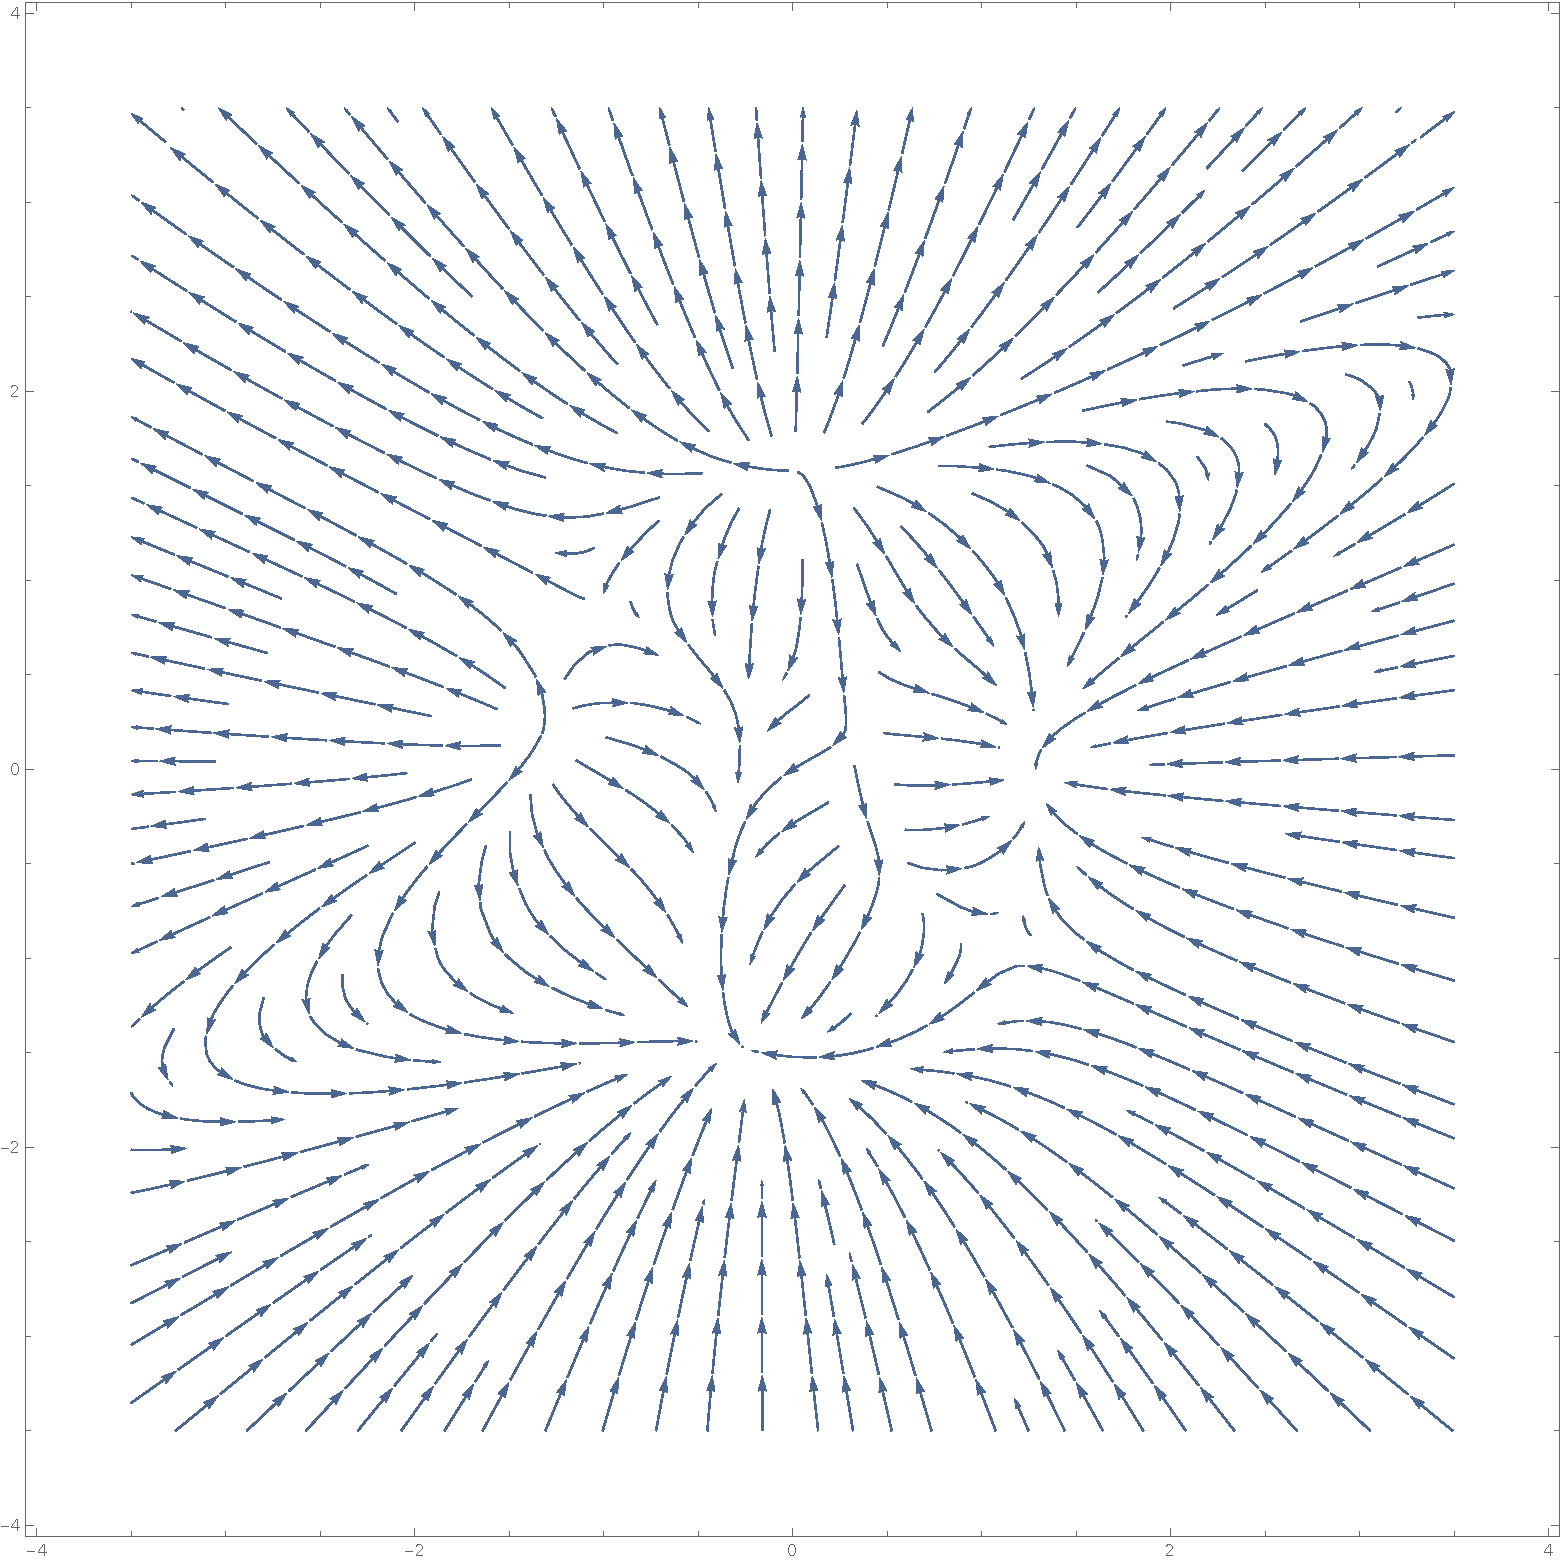
\includegraphics[keepaspectratio,height=5cm]{figures/vector-field.pdf}
    \caption{Wind Vector Field}
    \label{fig:wind}
  \end{figure}
\end{frame}

\begin{frame}{Underlying Scalar Function}
  \begin{figure}[h]
    \centering
    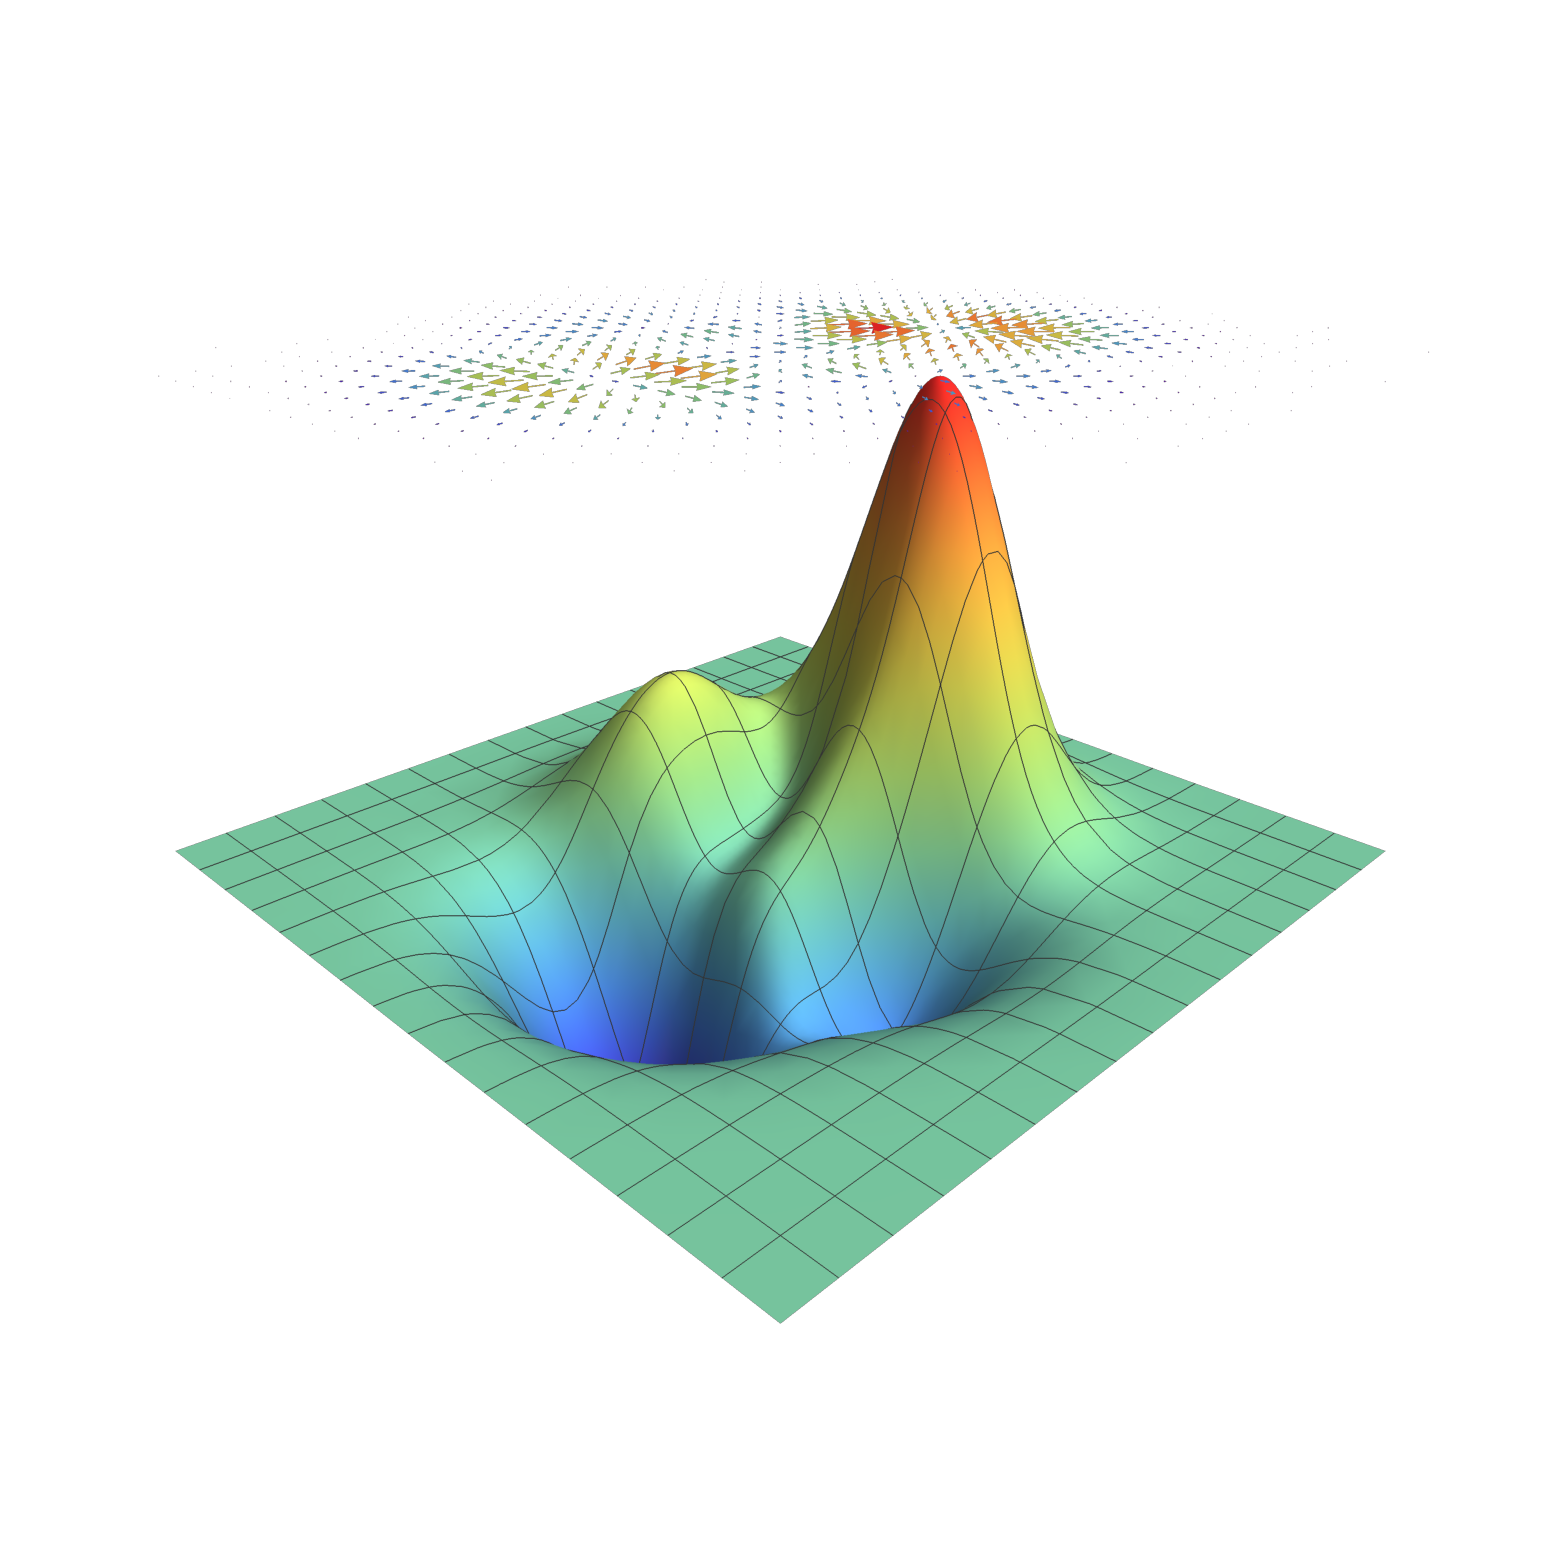
\includegraphics[keepaspectratio,height=7cm]{figures/vect-to-scalar.pdf}
  \end{figure}
\end{frame}

\begin{frame}{Shortest Time Path}
  \vfill
  \begin{figure}[h]
    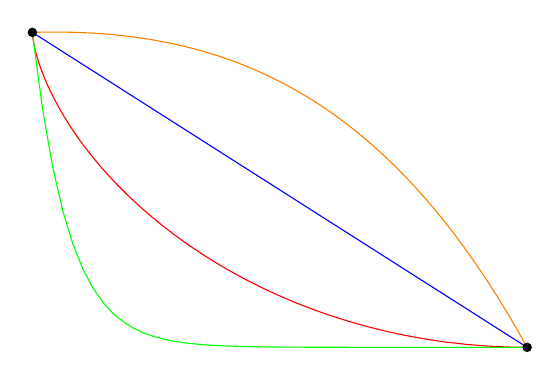
\begin{tikzpicture}[scale=2]
      \def\r{1} % radius
      \def\c{1.4} % center
      \coordinate (O) at (0,0);
      \coordinate (A) at (0,2*\r);
      \coordinate (B) at (pi, 0);

      % Cycloid
      \draw[red,domain=0:pi,samples=50] plot ({\x - sin(\x r)},{\r+cos(\x r)});

      % Straight line
      \draw[blue] (A) -- (B);

      % The other two
      \draw[green, domain=0:pi, samples=50] plot ({\x}, {(-2/pi)*(\x-pi)*exp(-4*\x)});
      \draw[orange, domain=0:pi, samples=50] plot ({\x}, {(-2/pi)*(\x-pi)*exp(\x/3)});

      % Release point
      \draw[fill=black] (A) circle (.75pt);

      % End point
      \draw[fill=black] (B) circle (.75pt);

    \end{tikzpicture}
  \end{figure}
  \vfill
\end{frame}


\begin{frame}{Shortest Path}
  \begin{figure}[h]
    \vfill
    \centering
    \definecolor{eek}{RGB}{255,255,255}
    \begin{tikzpicture}[
      scale=1.5,
      declare function = {
        a(\x, \y) = 3*(1-\x)^2 * exp(-(\x^2)-(\y+1)^2);
        b(\x, \y) = -10*(\x/5 - \x^3 + \y^5) * exp(-\x^2 - \y^2);
        c(\x, \y) = -exp(-(\x+1)^2 - \y^2)/3;
        Z(\x, \y) = a(\x,\y) + b(\x,\y) + c(\x,\y);
      }
      ]
      \begin{axis}[
        view={225}{50},
        hide x axis,
        hide y axis,
        hide z axis,
        domain=-3.5:3.5,
        samples=60,
        % grid=major,
        ]
        \addplot3 [surf] {Z(x,y)};
        \addplot3 [only marks, mark options={scale=.4}] table[row sep=crcr] {
          x y z \\
          1.5 2 -.558409 \\
          -.5 -1.5 10.2248 \\
        };

        \addplot3 [color=eek, line width=.3mm] table[row sep=crcr] {


          x y z\\
          1.5 2. -0.558409\\
          1.51642 1.94419 -0.563117\\
          1.5281 1.89109 -0.566764\\
          1.5359 1.8402 -0.568777\\
          1.54042 1.79119 -0.568625\\
          1.54169 1.74403 -0.566657\\
          1.53972 1.69873 -0.563314\\
          1.53448 1.6553 -0.559113\\
          1.52618 1.61361 -0.554089\\
          1.51513 1.57349 -0.547923\\
          1.50152 1.53485 -0.540551\\
          1.48554 1.49755 -0.531797\\
          1.46734 1.46152 -0.521699\\
          1.44696 1.42673 -0.51058\\
          1.4246 1.39308 -0.498421\\
          1.40039 1.36049 -0.485341\\
          1.37444 1.32889 -0.471672\\
          1.34694 1.29818 -0.45747\\
          1.31804 1.26827 -0.442899\\
          1.28794 1.23903 -0.427887\\
          1.25679 1.21041 -0.412675\\
          1.22478 1.18227 -0.397133\\
          1.19206 1.15454 -0.381331\\
          1.15877 1.12713 -0.365291\\
          1.12504 1.09997 -0.349063\\
          1.09101 1.073 -0.332668\\
          1.05677 1.04613 -0.316162\\
          1.02244 1.01932 -0.299556\\
          0.9881 0.992514 -0.282893\\
          0.953856 0.965654 -0.266204\\
          0.9198 0.938686 -0.249446\\
          0.886006 0.911568 -0.232734\\
          0.852562 0.88425 -0.216084\\
          0.819556 0.856682 -0.199503\\
          0.787085 0.828809 -0.182967\\
          0.755232 0.800582 -0.166606\\
          0.724107 0.771939 -0.150393\\
          0.69383 0.742811 -0.13433\\
          0.664525 0.713129 -0.118495\\
          0.636327 0.682813 -0.102999\\
          0.609409 0.651766 -0.0878422\\
          0.583954 0.619883 -0.0731155\\
          0.560159 0.587052 -0.0589631\\
          0.538254 0.55314 -0.045439\\
          0.518471 0.518016 -0.0326409\\
          0.501034 0.481552 -0.0206187\\
          0.486106 0.443654 -0.00944393\\
          0.47374 0.404291 0.000850495\\
          0.463844 0.363518 0.010356\\
          0.456166 0.321477 0.0193537\\

          0.450241 0.278434 0.0280568\\
          0.445477 0.234727 0.0366758\\
          0.441231 0.190725 0.0453312\\
          0.436844 0.146804 0.0539149\\
          0.431781 0.103268 0.0624314\\
          0.425606 0.0603679 0.0709817\\
          0.417988 0.0182925 0.0799664\\
          0.408481 -0.0227036 0.0898276\\
          0.396483 -0.0622763 0.10142\\
          0.380887 -0.0997925 0.116149\\
          0.36006 -0.13432 0.137445\\
          0.332543 -0.165025 0.173063\\
          0.300746 -0.193283 0.234018\\
          0.268338 -0.221193 0.324566\\
          0.235187 -0.248678 0.445548\\
          0.20141 -0.275806 0.59699\\
          0.167168 -0.302668 0.777934\\
          0.136 -0.331286 0.977181\\
          0.106559 -0.360891 1.19437\\
          0.0820837 -0.393334 1.41713\\
          0.061576 -0.428043 1.64678\\
          0.0445095 -0.46472 1.88526\\
          0.0319881 -0.503993 2.13105\\
          0.0167515 -0.541715 2.40786\\
          -0.00246576 -0.577162 2.7188\\
          -0.0211968 -0.612888 3.05117\\
          -0.0378337 -0.649809 3.40215\\
          -0.0535971 -0.68723 3.77539\\
          -0.0703844 -0.724066 4.17318\\
          -0.090463 -0.759021 4.59408\\
          -0.117055 -0.790254 5.03122\\
          -0.151035 -0.817266 5.46954\\
          -0.18931 -0.841823 5.89331\\
          -0.233485 -0.863009 6.28331\\
          -0.272369 -0.887218 6.65243\\
          -0.312082 -0.910953 6.9853\\
          -0.350098 -0.935658 7.28763\\
          -0.385309 -0.961966 7.56667\\
          -0.417406 -0.990054 7.82827\\
          -0.447291 -1.0194 8.06996\\
          -0.472559 -1.05139 8.31202\\
          -0.497481 -1.08358 8.52372\\
          -0.518539 -1.11798 8.73285\\
          -0.536287 -1.15426 8.93522\\
          -0.550977 -1.1923 9.12719\\
          -0.56236 -1.23222 9.30809\\
          -0.569452 -1.2746 9.48209\\
          -0.571202 -1.32003 9.65093\\
          -0.565304 -1.36983 9.82094\\
          -0.547243 -1.42658 10.0008\\
          -0.5 -1.5 10.2248\\
        };
      \end{axis}
    \end{tikzpicture}
    \vfill
  \end{figure}
\end{frame}

% Function:
% z = 3 * (1-x)^2 * exp(-(x^2) - (y+1)^2) - 10 * (x/5 - x^3 - y^5) * exp(-x^2 -
% y^2) - 1/3 * exp(-(x+1)^2 - y^2)



\begin{frame}{The statement}
  \begin{theorem}[Euler-Lagrange]
    Let $\Qq(t) : \RR \to \RR^n$ be a path. Then if $\Qq(t)$ is an
    extreme value of the functional
    \[
      S(\Qq) = \int_a^b \mc L\pn{t, \Qq(t), \dot{\Qq}(t)} \dd t
    \]
    then $\Qq$ is a solution to the differential equation
    \[
      \pd{\mc L}{\Qq} - \od{}{t} \pn{\pd{\mc L}{\dot{\Qq}}} = 0
    \]
  \end{theorem}
\end{frame}

\section{Proof Sketch}

\begin{frame}
  \begin{figure}[h]
    \centering
    \begin{tikzpicture}
      \pgfmathsetmacro{\xmin}{-.2};
      \pgfmathsetmacro{\ymin}{-.2};
      \pgfmathsetmacro{\xmax}{6};
      \pgfmathsetmacro{\ymax}{5};

      \pgfmathsetmacro{\extraforaxes}{.2};

      \pgfmathsetmacro{\epsilon}{.1};

      \draw[->] (\xmin,0) -- (\xmax+\extraforaxes, 0) node[below] {$x$};
      \draw[->] (0,\ymin) -- (0, \ymax+\extraforaxes) node[left] {$y$};

      \draw[domain=1.5:5.5, smooth, variable=\x, blue] plot ({\x-.5},
      {-1.7 + \x * (3.31667 + (-0.9 + 0.0833333 * \x) * \x)});

      \node[
      circle,
      draw=black,
      fill=white,
      inner sep=0pt,
      minimum size=5pt
      ] (y0) at (1, 1.56875) {};

      \node[
      circle,
      draw=black,
      fill=white,
      inner sep=0pt,
      minimum size=5pt
      ] (y1) at (5, 3.18126) {};

      % \draw[domain=\xmin:\xmax, smooth, variable=\x, blue] plot ({\x}, )

      % \draw[scale=0.5,domain=-3:3,smooth,variable=\x,blue] plot ({\x}, {\x*\x});
      % \draw[scale=0.5,domain=-3:3,smooth,variable=\y,red]  plot ({\y*\y}, {\y});
    \end{tikzpicture}
  \end{figure}
\end{frame}


% \section{Bibliography}
% \begin{frame}
%   \frametitle{References}
%   \bibliographystyle{alpha}
%   %   \bibliographystyle{IEEE}
%   \bibliography{aha.bib}
% \end{frame}

\end{document}


%%% Local Variables:
%%% TeX-master: t
%%% TeX-engine: default-shell-escape
%%% TeX-command-extra-option: -pdf
%%% End: